\documentclass[../../main]{subfiles}

\renewcommand\thesection{\arabic{section}}


\begin{document}

\section{Pest Prevention} \label{sec:}

\begin{minipage} {0.62\textwidth}
    \vspace{-0.8cm}

    Developed a smart insect trap using the ESP-EYE microcontroller and FOMO
    algorithm, achieving 96\% accuracy with low resource use. It enables
    real-time fruit fly detection, targeted pesticide application, and
    automatic trap replacement. This sustainable, hands-free solution improves
    crop protection and can adapt to other pests.

\end{minipage}
\hfill
\begin{minipage} {0.35\textwidth}
    \begin{center}
        \vspace{-1.2cm}
        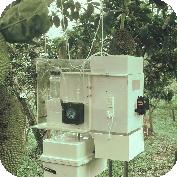
\includegraphics[width = 0.89\textwidth] {pics/trap.pdf}
        \captionof{figure}[Trap set up at the jackfruit orchard.]{}
        \label{fig:case3Pic}
    \end{center}
\end{minipage}

\subsection{What They Did}

In this study\cite{fruitfly}, Developed a TinyML based Fruit fly surveillance system,
implemented using ESP-EYE mircrocontroller. They used FOMO (Faster Objects,
More Objects) algorithm developed by the Edge Impulse platform.

\subsection{Results They Got}

The system performed with a maximum RAM usage of 2.4Mb and an inference time of
5.694 seconds. The FOMO model only required 53 kilo bytes of flash memory.
Furthermore, the trap ran smoothly without human intervention, thanks to its
automatic replacement feature for fly-stained adhesive traps


\end{document}
